\documentclass[11pt,a4paper]{article}
\usepackage[margin=1in]{geometry}
\usepackage{amsmath,amssymb}
\usepackage{graphicx}
\usepackage{enumitem}
\usepackage{tcolorbox}
\usepackage{array}
\usepackage{multirow}
\usepackage{tikz}
\usepackage{xcolor}
\usepackage{hyperref}
\usetikzlibrary{positioning,arrows.meta,shapes,calc}

% Colors
\definecolor{codegreen}{rgb}{0,0.6,0}
\definecolor{codegray}{rgb}{0.5,0.5,0.5}
\definecolor{codepurple}{rgb}{0.58,0,0.82}
\definecolor{backcolour}{rgb}{0.95,0.95,0.92}

% Custom commands
\newcommand{\highlight}[1]{\textbf{\color{blue}#1}}
\newcommand{\answer}[1]{\textcolor{blue}{\textit{#1}}}
\newcommand{\teaching}[1]{\textcolor{red}{\textbf{Teaching Note: }#1}}
\newcommand{\checkbox}{$\Box$}

% Environment definitions
\newtcolorbox{exercise}[1][]{
    colback=blue!5!white,
    colframe=blue!75!black,
    title=#1,
    fonttitle=\bfseries
}

\newtcolorbox{checkpoint}[1][]{
    colback=yellow!10!white,
    colframe=orange!75!black,
    title=Checkpoint,
    fonttitle=\bfseries
}

\newtcolorbox{discovery}[1][]{
    colback=green!5!white,
    colframe=green!75!black,
    title=Discovery Moment,
    fonttitle=\bfseries
}

\newtcolorbox{think}[1][]{
    colback=purple!5!white,
    colframe=purple!75!black,
    title=Think About It,
    fonttitle=\bfseries
}

\newtcolorbox{realworld}[1][]{
    colback=orange!5!white,
    colframe=orange!75!black,
    title=Real World Application,
    fonttitle=\bfseries
}

\newtcolorbox{warning}[1][]{
    colback=red!5!white,
    colframe=red!75!black,
    title=Common Pitfall,
    fonttitle=\bfseries
}

\newtcolorbox{teachingnote}[1][]{
    colback=red!5!white,
    colframe=red!75!black,
    title=Teaching Note,
    fonttitle=\bfseries
}

% Title and header
\title{\textbf{Word Embeddings in 3D: Post-Class Learning Verification}\\
\large Checking Your Understanding After the Interactive Lab\\
\vspace{0.5em}
\large \textit{From Words to Vectors: Can You Apply What You Learned?}\\
\vspace{0.5em}
\textcolor{red}{\textbf{INSTRUCTOR VERSION WITH ANSWER KEY}}}
\author{NLP Course 2025 - BSc Level Assessment}
\date{}

\begin{document}
\maketitle

\noindent\textbf{Time Required:} 45-60 minutes\\
\textbf{Purpose:} Verify and deepen your understanding of word embeddings after completing the interactive notebook\\
\textbf{Format:} No coding required - focus on concepts, visualization, and application

\begin{teachingnote}
This assessment is designed to verify learning after students complete the interactive notebook. Encourage discussion and peer learning. Students often struggle with the vector arithmetic concept - use physical analogies (directions in space) if needed.
\end{teachingnote}

\begin{checkpoint}
\textbf{Before Starting:} You should have completed the ``word\_embeddings\_3d\_bsc.ipynb'' notebook. This handout will test your understanding of:
\begin{itemize}
    \item Why words need to be vectors
    \item How Word2Vec learns from context
    \item Word similarity and clustering
    \item Word arithmetic
    \item Applications of embeddings
\end{itemize}
\end{checkpoint}

\hrule
\vspace{1em}

\section*{Part A: Conceptual Understanding \hfill (20 minutes)}

\teaching{This section tests foundational understanding. Look for evidence that students grasp the core concept of distributed representation.}

\subsection*{A1: The Embedding Concept (5 minutes)}

\begin{exercise}[Why Vectors?]
\textbf{Question 1:} Explain in your own words why computers need word embeddings instead of just treating words as text strings.

\answer{Computers need numerical representations to perform calculations. Text strings can't be compared mathematically or used in machine learning algorithms. Embeddings convert words to vectors where:
- Similar meanings have similar vectors (measurable with cosine similarity)
- Mathematical operations become possible (addition, subtraction)
- Machine learning models can process them (neural networks need numbers)
- Relationships between words become computable}

\textbf{Question 2:} Draw simple 2D vectors for these words showing their relationships:
\begin{itemize}
    \item cat, dog, car
    \item Show which two should be closer together and why
\end{itemize}

\begin{center}
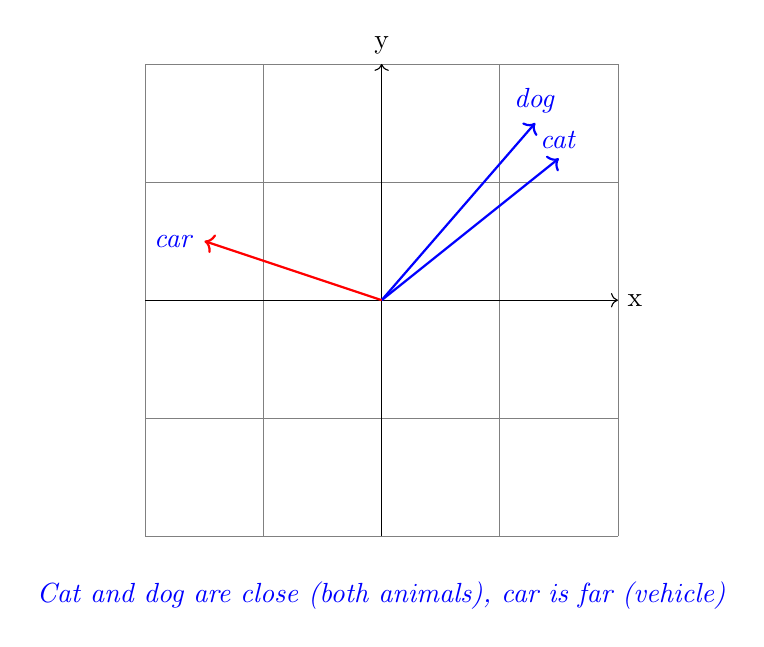
\begin{tikzpicture}[scale=1.5]
    % Grid
    \draw[gray, very thin] (-2,-2) grid (2,2);
    \draw[->] (-2,0) -- (2,0) node[right] {x};
    \draw[->] (0,-2) -- (0,2) node[above] {y};
    
    % Answer vectors
    \draw[->, thick, blue] (0,0) -- (1.5,1.2) node[above] {\answer{cat}};
    \draw[->, thick, blue] (0,0) -- (1.3,1.5) node[above] {\answer{dog}};
    \draw[->, thick, red] (0,0) -- (-1.5,0.5) node[left] {\answer{car}};
    
    \node[blue] at (0,-2.5) {\answer{Cat and dog are close (both animals), car is far (vehicle)}};
\end{tikzpicture}
\end{center}

\textbf{Visualization:} Real 3D Word Embedding Space
\begin{center}
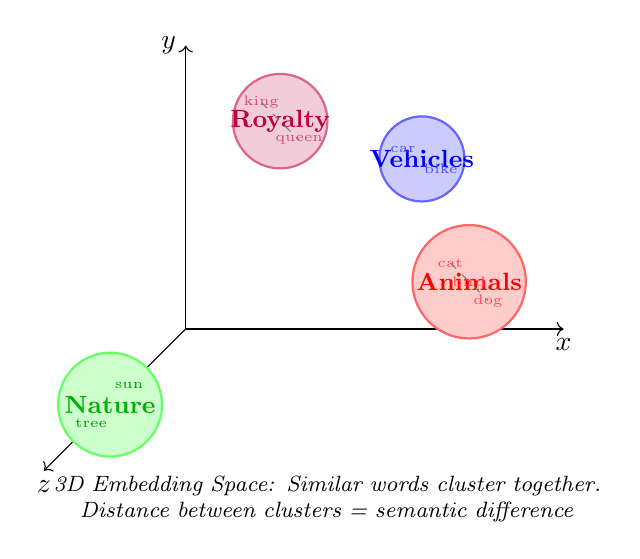
\begin{tikzpicture}[scale=1.2]
    % Pseudo-3D axes
    \draw[->] (0,0) -- (4,0) node[anchor=north]{$x$};
    \draw[->] (0,0) -- (0,3) node[anchor=east]{$y$};
    \draw[->] (0,0) -- (-1.5,-1.5) node[anchor=north]{$z$};
    
    % Animal cluster (red circle)
    \draw[red!60,fill=red!20,thick] (3,0.5) circle (0.6cm);
    \node[red,font=\small\bfseries] at (3,0.5) {Animals};
    \node[red!70,font=\tiny] at (2.8,0.7) {cat};
    \node[red!70,font=\tiny] at (3.2,0.3) {dog};
    \node[red!70,font=\tiny] at (3,0.5) {bird};
    
    % Royalty cluster (purple circle)  
    \draw[purple!60,fill=purple!20,thick] (1,2.2) circle (0.5cm);
    \node[purple,font=\small\bfseries] at (1,2.2) {Royalty};
    \node[purple!70,font=\tiny] at (0.8,2.4) {king};
    \node[purple!70,font=\tiny] at (1.2,2.0) {queen};
    
    % Nature cluster (green circle)
    \draw[green!60,fill=green!20,thick] (-0.8,-0.8) circle (0.55cm);
    \node[green!70!black,font=\small\bfseries] at (-0.8,-0.8) {Nature};
    \node[green!60!black,font=\tiny] at (-0.6,-0.6) {sun};
    \node[green!60!black,font=\tiny] at (-1.0,-1.0) {tree};
    
    % Vehicle cluster (blue circle)
    \draw[blue!60,fill=blue!20,thick] (2.5,1.8) circle (0.45cm);
    \node[blue,font=\small\bfseries] at (2.5,1.8) {Vehicles};
    \node[blue!70,font=\tiny] at (2.3,1.9) {car};
    \node[blue!70,font=\tiny] at (2.7,1.7) {bike};
    
    % Draw connections between similar words
    \draw[dashed,gray,thin] (2.8,0.7) -- (3.2,0.3);
    \draw[dashed,gray,thin] (0.8,2.4) -- (1.2,2.0);
    
    % Legend
    \node[font=\footnotesize,text width=7cm,align=center] at (1.5,-1.8) {
        \textit{3D Embedding Space: Similar words cluster together.\\
        Distance between clusters = semantic difference}
    };
\end{tikzpicture}
\end{center}

\textbf{Question 3:} Circle the TRUE statements:
\begin{itemize}
    \item[\answer{\checkmark}] Embeddings capture word meaning as numbers
    \item[\answer{\checkmark}] Similar words have similar vectors
    \item[\checkbox] Each word gets exactly one dimension \answer{FALSE - each word has MANY dimensions}
    \item[\answer{\checkmark}] Context determines embedding values
    \item[\checkbox] Embeddings are always 3D \answer{FALSE - typically 50-300 dimensions}
\end{itemize}

\teaching{Common misconception: Students often confuse "dimension" with "one number per word". Clarify that each word is a point in n-dimensional space.}
\end{exercise}

\subsection*{A2: Context Windows (5 minutes)}

\begin{exercise}[Understanding Context]
Given the sentence: \textbf{``The quick brown fox jumps over the lazy dog''}

\textbf{Task 1:} If we're training on the word ``fox'' with window size = 2, circle all context words:

\begin{center}
The \quad \answer{\fbox{quick}} \quad \answer{\fbox{brown}} \quad \boxed{fox} \quad \answer{\fbox{jumps}} \quad \answer{\fbox{over}} \quad the \quad lazy \quad dog
\end{center}

\teaching{Window size = 2 means 2 words before AND 2 words after. Students often forget it's bidirectional.}

\textbf{Task 2:} How would changing window size affect learning?

\begin{tabular}{|l|p{8cm}|}
\hline
Window = 1 & \answer{Captures immediate syntactic relationships (adjective-noun, verb-object). Good for grammar but misses broader meaning.} \\
\hline
Window = 5 & \answer{Captures both syntax and broader semantic context. Balanced approach for most applications.} \\
\hline
Window = 10 & \answer{Captures document-level themes and topics but dilutes local syntactic patterns. May include unrelated words.} \\
\hline
\end{tabular}

\textbf{Task 3:} Which window size would be better for:
\begin{itemize}
    \item Learning syntax (grammar): \answer{Small (1-2) - captures immediate dependencies}
    \item Learning topic/theme: \answer{Large (5-10) - captures broader context}
\end{itemize}
\end{exercise}

\subsection*{A3: Dimensions and Quality (5 minutes)}

\begin{exercise}[Dimension Trade-offs]
\textbf{Scenario:} You're choosing embedding dimensions for different applications.

\textbf{Task 1:} Match the dimension size to the use case:
\begin{center}
\begin{tabular}{|l|l|}
\hline
\textbf{Application} & \textbf{Suggested Dimensions} \\
\hline
Simple word similarity & \answer{10-50} \\
\hline
Complex language model & \answer{100-300} \\
\hline
Visualization in 3D & \answer{exactly 3} \\
\hline
Mobile app (limited memory) & \answer{10-50} \\
\hline
Research with huge vocabulary & \answer{500+} \\
\hline
\end{tabular}
\end{center}

\textbf{Task 2:} Explain the trade-off:
\begin{itemize}
    \item More dimensions = \answer{Better representation, captures more nuances, but requires more memory and computation}
    \item Fewer dimensions = \answer{Faster, less memory, but may lose important distinctions between words}
\end{itemize}

\teaching{Use the analogy of describing a person: 3 features (height, weight, age) vs. 100 features - more features = better description but harder to process.}
\end{exercise}

\subsection*{A4: Quick Concept Check (5 minutes)}

\begin{think}
Rate your understanding (1 = confused, 5 = confident):
\begin{itemize}
    \item[\checkbox] Words as vectors \hfill [1] [2] [3] [4] [5]
    \item[\checkbox] Context windows \hfill [1] [2] [3] [4] [5]
    \item[\checkbox] Training process \hfill [1] [2] [3] [4] [5]
    \item[\checkbox] Similarity measurement \hfill [1] [2] [3] [4] [5]
\end{itemize}

\teaching{Students rating below 3 need additional support. Consider peer tutoring or office hours.}
\end{think}

\newpage

\section*{Part B: Practical Application \hfill (15 minutes)}

\teaching{This section tests ability to apply concepts. Watch for students who understand theory but struggle with application.}

\subsection*{B1: Word Similarity Exercise (5 minutes)}

\begin{exercise}[Computing Similarity]
Given these simplified 3D embeddings:
\begin{itemize}
    \item king = [0.8, 0.2, 0.5]
    \item queen = [0.7, 0.3, 0.6]
    \item car = [0.1, 0.9, 0.2]
\end{itemize}

\textbf{Task 1:} Which pair is more similar? (Use rough estimation)
\begin{itemize}
    \item king \& queen: Distance $\approx$ \answer{0.17 (very close)}
    \item king \& car: Distance $\approx$ \answer{0.92 (far apart)}
    \item More similar pair: \answer{king \& queen}
\end{itemize}

\teaching{Don't require exact calculations. Looking for understanding that smaller distance = more similar.}

\textbf{Task 2:} Rank these word pairs by expected similarity (1 = most similar):
\begin{itemize}
    \item[\answer{4}] cat - dog
    \item[\answer{3}] king - queen  
    \item[\answer{5}] happy - sad
    \item[\answer{1}] computer - laptop
    \item[\answer{6}] run - blue
\end{itemize}

\textbf{Task 3:} Draw approximate clusters:
\begin{center}
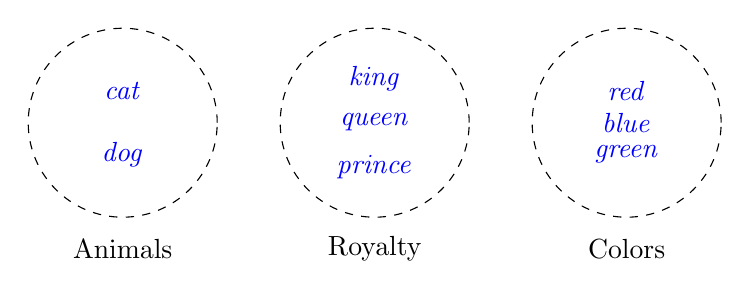
\begin{tikzpicture}[scale=0.8]
    % Draw circles for clusters
    \draw[dashed] (0,0) circle (1.5cm);
    \node at (0,-2) {Animals};
    \node[blue] at (0,0.5) {\answer{cat}};
    \node[blue] at (0,-0.5) {\answer{dog}};
    
    \draw[dashed] (4,0) circle (1.5cm);
    \node at (4,-2) {Royalty};
    \node[purple] at (4,0.7) {\answer{king}};
    \node[purple] at (4,0) {\answer{queen}};
    \node[purple] at (4,-0.7) {\answer{prince}};
    
    \draw[dashed] (8,0) circle (1.5cm);
    \node at (8,-2) {Colors};
    \node[green] at (8,0.5) {\answer{red}};
    \node[green] at (8,0) {\answer{blue}};
    \node[green] at (8,-0.5) {\answer{green}};
\end{tikzpicture}
\end{center}
\end{exercise}

\subsection*{B2: Word Arithmetic Magic (5 minutes)}

\begin{exercise}[Vector Math with Words]
\textbf{Task 1:} Complete these analogies:
\begin{itemize}
    \item king - man + woman = \answer{queen}
    \item paris - france + germany = \answer{berlin}
    \item cat - kitten + puppy = \answer{dog}
\end{itemize}

\textbf{Task 2:} Create your own word equation:

\answer{Example: doctor - man + woman = nurse (Note: This reveals gender bias in embeddings!)}

\teaching{Use this as an opportunity to discuss bias in embeddings - they reflect biases in training data.}

\textbf{Task 3:} Draw the vector arithmetic for: ``summer - hot + cold''

\begin{center}
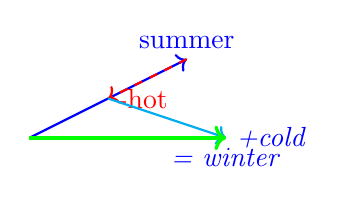
\begin{tikzpicture}[scale=1]
    % Start with summer vector
    \draw[->, thick, blue] (0,0) -- (2,1) node[above] {summer};
    
    % Subtract hot
    \draw[->, thick, red, dashed] (2,1) -- (1,0.5) node[right] {-hot};
    
    % Add cold
    \draw[->, thick, cyan] (1,0.5) -- (2.5,0) node[right] {\answer{+cold}};
    
    % Result
    \draw[->, thick, green, very thick] (0,0) -- (2.5,0) node[below] {\answer{= winter}};
\end{tikzpicture}
\end{center}

\textbf{Task 4:} Explain why word arithmetic works:

\answer{Word vectors encode semantic relationships as geometric directions. The vector from "man" to "king" represents "royalty" or "leadership". Adding this same direction to "woman" gives "queen". The relationships are consistent across the vector space.}
\end{exercise}

\subsection*{B3: 3D Visualization Interpretation (5 minutes)}

\begin{exercise}[Reading 3D Plots]
Imagine you see a 3D plot where:
\begin{itemize}
    \item ``love'' and ``hate'' are far apart
    \item ``cat'' and ``dog'' are close together
    \item ``king'' and ``queen'' form a cluster with ``prince''
\end{itemize}

\textbf{Task 1:} What does distance represent in the plot?

\answer{Semantic similarity - the closer two words are in the embedding space, the more similar their meaning/usage in the training corpus.}

\textbf{Task 2:} Where would you expect to find these words?
\begin{itemize}
    \item ``affection'' - Near: \answer{love (positive emotion)}
    \item ``princess'' - Near: \answer{royalty cluster (king/queen/prince)}
    \item ``fish'' - Near: \answer{cat/dog (animals cluster)}
\end{itemize}

\textbf{Task 3:} If words gradually move closer during training, what's happening?

\answer{The model is learning that these words appear in similar contexts and have related meanings. The training process adjusts vectors to minimize prediction error, bringing similar words together.}

\teaching{Use the metaphor of "words finding their neighborhood" during training.}
\end{exercise}

\newpage

\section*{Part C: Hands-On Problem Solving \hfill (15 minutes)}

\teaching{This section requires synthesis and creative thinking. Encourage students to explain their reasoning.}

\subsection*{C1: Build Your Own Embeddings (5 minutes)}

\begin{exercise}[Design Embeddings from Scratch]
Given these 5 sentences:
\begin{enumerate}
    \item The cat sleeps
    \item The dog plays
    \item Cats and dogs play
    \item Birds fly high
    \item Fish swim deep
\end{enumerate}

\textbf{Task 1:} Create word-context pairs for ``cat'' (window=1):
\begin{itemize}
    \item Context words: \answer{The, sleeps (from sentence 1)}
    \item Context words: \answer{Cats, and (from sentence 3)}
\end{itemize}

\textbf{Task 2:} Design simple 2D vectors for these words:
\begin{center}
\begin{tabular}{|l|c|c|}
\hline
\textbf{Word} & \textbf{x} & \textbf{y} \\
\hline
cat & \answer{0.7} & \answer{0.5} \\
\hline
dog & \answer{0.8} & \answer{0.6} \\
\hline
bird & \answer{0.6} & \answer{0.7} \\
\hline
fish & \answer{0.5} & \answer{0.4} \\
\hline
\end{tabular}
\end{center}

\answer{Note: All animals should have similar values, clustering them together}

\textbf{Task 3:} Which words should cluster together? Why?

\answer{All four animals (cat, dog, bird, fish) should cluster together as they're all animals and appear in similar grammatical structures. "The" would be separate (determiner), and action verbs (sleeps, plays, fly, swim) might form another cluster.}
\end{exercise}

\subsection*{C2: Application Design (5 minutes)}

\begin{exercise}[Building with Embeddings]
\textbf{Task 1:} Design a synonym finder:

\begin{enumerate}
    \item Input: \answer{A word (string)}
    \item Process: \answer{Convert to embedding, compute cosine similarity with all other word vectors, sort by similarity}
    \item Output: \answer{Top 5-10 most similar words}
\end{enumerate}

\textbf{Task 2:} Sketch a sentiment analyzer:

How would you use embeddings to determine if text is positive/negative?

\answer{Average the embeddings of all words in the text to get a document vector. Train a classifier on labeled examples where positive and negative texts should have different average embeddings. Or compute similarity to known positive/negative word lists.}

\teaching{There are multiple valid approaches. Look for understanding that embeddings can be aggregated and classified.}

\textbf{Task 3:} Your creative application:

Design a new use for word embeddings:
\begin{itemize}
    \item Name: \answer{Example: "Story Coherence Checker"}
    \item Purpose: \answer{Detect when a story goes off-topic by tracking embedding distances between sentences}
    \item How embeddings help: \answer{Sudden large distances between consecutive sentence embeddings indicate topic shifts}
\end{itemize}
\end{exercise}

\subsection*{C3: Debugging Scenarios (5 minutes)}

\begin{warning}
Real problems you might encounter:
\end{warning}

\begin{exercise}[Problem Solving]
\textbf{Scenario 1:} The word ``bank'' appears near both ``river'' and ``money''. 
\begin{itemize}
    \item Problem: \answer{Polysemy - one word with multiple meanings gets a single averaged embedding}
    \item Solution: \answer{Use contextual embeddings (BERT) or sense-specific embeddings}
\end{itemize}

\textbf{Scenario 2:} A new word ``COVID'' doesn't exist in your embeddings.
\begin{itemize}
    \item Problem: \answer{Out-of-vocabulary (OOV) word - not seen during training}
    \item Solution: \answer{Use subword tokenization, character-level models, or retrain with updated corpus}
\end{itemize}

\textbf{Scenario 3:} Your embeddings show ``doctor''=male, ``nurse''=female bias.
\begin{itemize}
    \item Problem: \answer{Training data bias reflected in embeddings}
    \item Solution: \answer{Debiasing techniques: neutralize gender direction, augment training data, or use fairness constraints}
\end{itemize}

\teaching{These scenarios open discussions about real-world challenges in NLP deployment.}
\end{exercise}

\newpage

\section*{Part D: Reflection \& Extension \hfill (10 minutes)}

\subsection*{D1: Self-Assessment Checklist (3 minutes)}

\begin{checkpoint}
Check off what you can now do:
\begin{itemize}
    \item[\checkbox] Explain why words need to be vectors \answer{Core concept}
    \item[\checkbox] Describe how Word2Vec learns from context \answer{CBOW/Skip-gram}
    \item[\checkbox] Calculate word similarity (roughly) \answer{Distance/cosine}
    \item[\checkbox] Perform word arithmetic \answer{Vector operations}
    \item[\checkbox] Identify word clusters in 3D space \answer{Visualization}
    \item[\checkbox] Design applications using embeddings \answer{Practical use}
    \item[\checkbox] Recognize common problems and solutions \answer{Debugging}
\end{itemize}

\teaching{Students checking fewer than 5 items need additional review. Consider remedial exercises.}
\end{checkpoint}

\subsection*{D2: Real-World Connections (3 minutes)}

\begin{realworld}
\textbf{Connect to Industry:}
\begin{enumerate}
    \item How does Google use embeddings in search?
    
    \answer{Google uses embeddings to understand query intent, find semantically similar pages even without exact keyword matches, and improve search relevance through semantic search.}
    
    \item How do embeddings connect to ChatGPT/BERT?
    
    \answer{These models use contextual embeddings where the same word gets different vectors based on context. They build on Word2Vec concepts but add attention mechanisms and transformer architectures.}
    
    \item Name one ethical concern with embeddings:
    
    \answer{Bias amplification - embeddings trained on biased data perpetuate stereotypes (gender, race, etc.) in downstream applications.}
\end{enumerate}
\end{realworld}

\subsection*{D3: Challenge Questions (4 minutes)}

\begin{think}
\textbf{Going Deeper:}
\begin{enumerate}
    \item Could we create embeddings for images? How?
    
    \answer{Yes! Convolutional Neural Networks (CNNs) create image embeddings where similar images have similar vectors. The last hidden layer before classification serves as the embedding.}
    
    \item What about embedding DNA sequences or music?
    
    \answer{DNA: Treat nucleotides as "words" and sequences as "sentences". Music: Embed notes/chords as words, or use spectrograms. Both use sequence modeling techniques similar to Word2Vec.}
    
    \item How would you embed an entire document (not just words)?
    
    \answer{Options: (1) Average all word embeddings, (2) Use Doc2Vec which learns document-specific vectors, (3) Use BERT's [CLS] token, (4) Weighted average based on TF-IDF.}
\end{enumerate}

\teaching{These extension questions can lead to research projects or advanced coursework discussions.}
\end{think}

\hrule
\vspace{1em}

\section*{Final Reflection}

\begin{discovery}
\textbf{The Big Picture:}

You've learned that word embeddings transform language into mathematical space where:
\begin{itemize}
    \item Meaning becomes measurable
    \item Relationships become computable
    \item Patterns become visible
\end{itemize}

This is the foundation of modern NLP - from search engines to chatbots to translation systems!
\end{discovery}

\vspace{1em}

\textbf{Areas needing review?} List them here:
\begin{itemize}
    \item \answer{Common issues: word arithmetic intuition, dimension selection, bias understanding}
    \item \answer{Suggest targeted exercises based on gaps}
    \item \answer{Point to specific notebook sections for review}
\end{itemize}

\vspace{1em}

\textbf{Most interesting discovery:} \answer{Look for genuine engagement and curiosity - these students may benefit from research opportunities}

\vspace{1em}

\textbf{One question you still have:} \answer{Address in next class or office hours - common questions become teaching opportunities}

\hrule
\vspace{1em}

\section*{Grading Rubric}

\begin{teachingnote}
\textbf{Point Distribution (Total: 100 points)}
\begin{itemize}
    \item Part A: 30 points (Conceptual understanding)
    \item Part B: 25 points (Practical application)  
    \item Part C: 30 points (Problem solving)
    \item Part D: 15 points (Reflection and extension)
\end{itemize}

\textbf{Partial Credit Guidelines:}
\begin{itemize}
    \item Correct reasoning with minor errors: 75\% credit
    \item Right approach, wrong conclusion: 50\% credit
    \item Attempted but incorrect: 25\% credit
\end{itemize}

\textbf{Common Errors to Watch For:}
\begin{itemize}
    \item Confusing embedding dimensions with vocabulary size
    \item Not understanding bidirectional context windows
    \item Thinking embeddings are always positive numbers
    \item Missing the connection between distance and similarity
\end{itemize}
\end{teachingnote}

\section*{Next Steps}

\begin{itemize}
    \item Review sections with ratings below 3
    \item Try coding your own Word2Vec model
    \item Explore pre-trained embeddings (GloVe, FastText)
    \item Learn about contextual embeddings (BERT)
    \item Apply embeddings to a real project
\end{itemize}

\teaching{Encourage students to implement a small project using embeddings - this solidifies understanding better than any exercise.}

\vspace{2em}
\begin{center}
\textbf{--- End of Assessment ---}
\end{center}

\end{document}